% Figure: Astrocyte-Neuron Lactate Shuttle (ANLS) Dysfunction
% Shows proposed mechanism for CNS-specific energy failure

\begin{figure}[htbp]
\centering
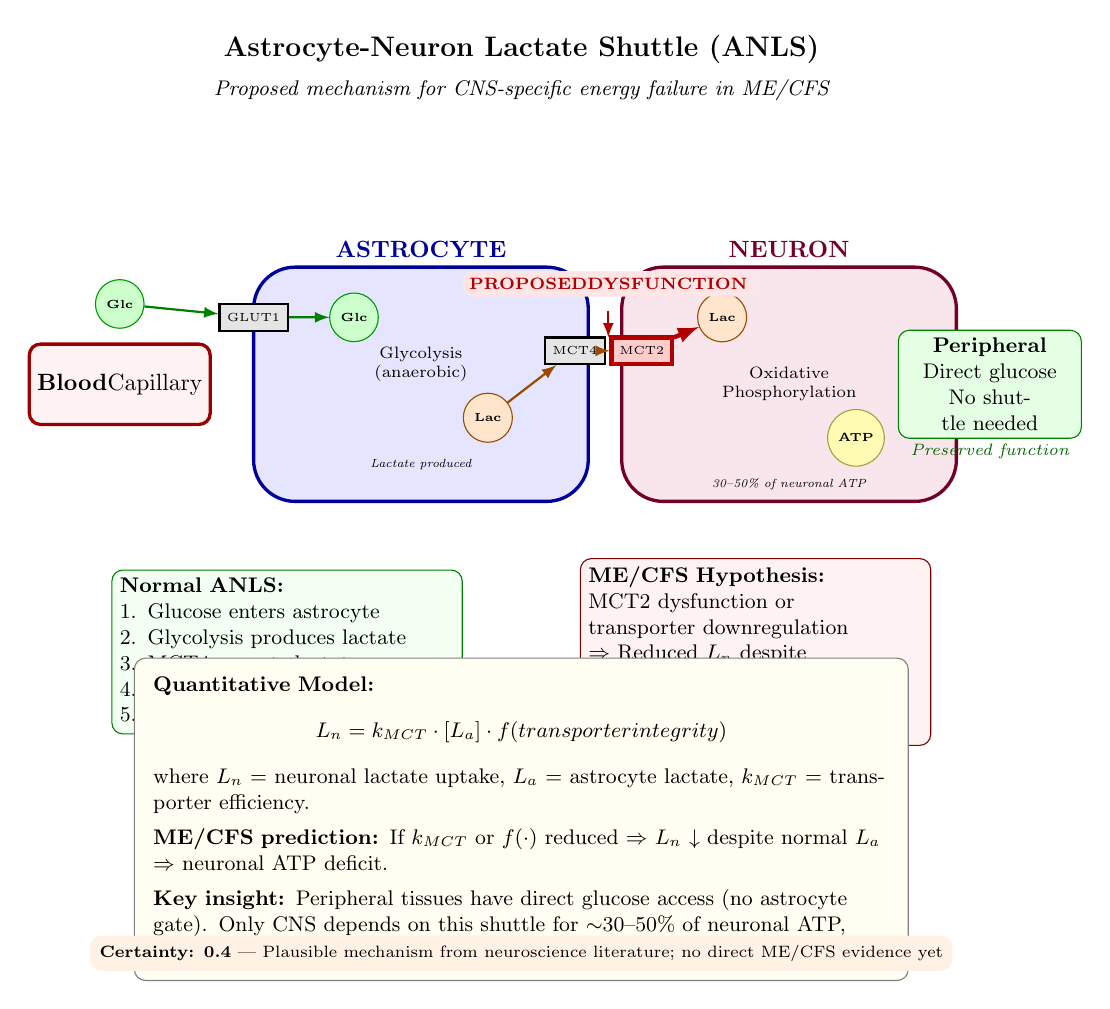
\begin{tikzpicture}[
    scale=0.85, every node/.style={scale=0.85},
    % Cell styles
    astrocyte/.style={draw=blue!60!black, fill=blue!10, very thick, rounded corners=15pt, minimum width=5cm, minimum height=3.5cm},
    neuron/.style={draw=purple!60!black, fill=purple!10, very thick, rounded corners=15pt, minimum width=5cm, minimum height=3.5cm},
    capillary/.style={draw=red!60!black, fill=red!5, very thick, rounded corners, minimum width=2cm, minimum height=1.2cm},
    % Molecule styles
    glucose/.style={circle, draw=green!60!black, fill=green!20, minimum size=0.6cm, font=\tiny\bfseries},
    lactate/.style={circle, draw=orange!60!black, fill=orange!20, minimum size=0.6cm, font=\tiny\bfseries},
    atp/.style={circle, draw=yellow!60!black, fill=yellow!30, minimum size=0.6cm, font=\tiny\bfseries},
    % Transporter styles
    transporter/.style={draw=black, fill=gray!20, thick, minimum width=0.8cm, minimum height=0.4cm, font=\tiny},
    transporter-impaired/.style={draw=red!70!black, fill=red!20, ultra thick, minimum width=0.8cm, minimum height=0.4cm, font=\tiny},
    % Arrow styles
    flow/.style={-latex, thick, green!50!black},
    flow-impaired/.style={-latex, very thick, red!70!black, dashed},
    shuttle/.style={-latex, thick, orange!60!black},
    shuttle-impaired/.style={-latex, ultra thick, red!70!black, dashed},
]

% Title
\node[font=\large\bfseries] at (0, 8) {Astrocyte-Neuron Lactate Shuttle (ANLS)};
\node[font=\small\itshape] at (0, 7.4) {Proposed mechanism for CNS-specific energy failure in ME/CFS};

% === BLOOD CAPILLARY ===
\node[capillary] (cap) at (-6, 3) {\textbf{Blood}\\Capillary};
\node[glucose] (gluc-blood) at (-6, 4.2) {Glc};

% === ASTROCYTE ===
\node[astrocyte, label={[font=\bfseries, blue!60!black]above:ASTROCYTE}] (astro) at (-1.5, 3) {};

% Astrocyte contents
\node[glucose] (gluc-astro) at (-2.5, 4) {Glc};
\node[font=\scriptsize, text width=2cm, align=center] at (-1.5, 3.3) {Glycolysis\\(anaerobic)};
\node[lactate] (lac-astro) at (-0.5, 2.5) {Lac};
\node[font=\tiny\itshape] at (-1.5, 1.8) {Lactate produced};

% Glucose transporter (BBB to astrocyte)
\node[transporter] (glut1) at (-4, 4) {GLUT1};
\draw[flow] (gluc-blood) -- (glut1);
\draw[flow] (glut1) -- (gluc-astro);

% === NEURON ===
\node[neuron, label={[font=\bfseries, purple!60!black]above:NEURON}] (neur) at (4, 3) {};

% Neuron contents
\node[lactate] (lac-neur) at (3, 4) {Lac};
\node[font=\scriptsize, text width=2cm, align=center] at (4, 3) {Oxidative\\Phosphorylation};
\node[atp] (atp-neur) at (5, 2.2) {ATP};
\node[font=\tiny\itshape] at (4, 1.5) {30--50\% of neuronal ATP};

% === MCT TRANSPORTERS (key site) ===
% Astrocyte MCT4 (lactate export)
\node[transporter] (mct4) at (0.8, 3.5) {MCT4};
\draw[shuttle] (lac-astro) -- (mct4);

% Neuron MCT2 (lactate import) - POTENTIALLY IMPAIRED
\node[transporter-impaired] (mct2) at (1.8, 3.5) {MCT2};
\draw[shuttle] (mct4) -- (mct2);
\draw[shuttle-impaired] (mct2) -- (lac-neur);

% Impairment indicator
\node[font=\scriptsize\bfseries, red!70!black, fill=red!10, rounded corners, inner sep=3pt] at (1.3, 4.5) {PROPOSED\\DYSFUNCTION};
\draw[-latex, red!70!black, thick] (1.3, 4.1) -- (1.3, 3.7);

% === NORMAL PATHWAY ANNOTATION ===
\begin{scope}[yshift=-1cm]
    \node[draw=green!50!black, fill=green!5, rounded corners, text width=5cm, align=left, font=\small] at (-3.5, 0) {
    \textbf{Normal ANLS:}\\
    1. Glucose enters astrocyte\\
    2. Glycolysis produces lactate\\
    3. MCT4 exports lactate\\
    4. MCT2 imports to neuron\\
    5. Oxidative phos. $\rightarrow$ ATP
    };
\end{scope}

% === ME/CFS HYPOTHESIS ANNOTATION ===
\begin{scope}[yshift=-1cm]
    \node[draw=red!50!black, fill=red!5, rounded corners, text width=5cm, align=left, font=\small] at (3.5, 0) {
    \textbf{ME/CFS Hypothesis:}\\
    MCT2 dysfunction or\\
    transporter downregulation\\
    $\Rightarrow$ Reduced $L_n$ despite\\
    \hspace{6pt} normal $L_a$\\
    $\Rightarrow$ CNS-specific energy\\
    \hspace{6pt} deficit
    };
\end{scope}

% === EQUATIONS ===
\node[draw=black!50, fill=yellow!5, rounded corners, text width=11cm, align=left, font=\small, inner sep=8pt] at (0, -3.5) {
\textbf{Quantitative Model:}
\[
L_n = k_{MCT} \cdot [L_a] \cdot f(\text{transporter integrity})
\]
where $L_n$ = neuronal lactate uptake, $L_a$ = astrocyte lactate, $k_{MCT}$ = transporter efficiency.\\[4pt]
\textbf{ME/CFS prediction:} If $k_{MCT}$ or $f(\cdot)$ reduced $\Rightarrow$ $L_n \downarrow$ despite normal $L_a$ $\Rightarrow$ neuronal ATP deficit.\\[4pt]
\textbf{Key insight:} Peripheral tissues have direct glucose access (no astrocyte gate). Only CNS depends on this shuttle for $\sim$30--50\% of neuronal ATP, explaining CNS-specific vulnerability.
};

% === PERIPHERAL COMPARISON ===
\begin{scope}[xshift=7cm, yshift=3cm]
    \node[draw=green!50!black, fill=green!10, rounded corners, text width=2.5cm, align=center, font=\small] (periph) at (0, 0) {\textbf{Peripheral}\\Direct glucose\\No shuttle needed};
    \node[font=\scriptsize\itshape, green!40!black] at (0, -1) {Preserved function};
\end{scope}

% === CERTAINTY ===
\node[font=\scriptsize, fill=orange!10, rounded corners, inner sep=4pt] at (0, -5.5) {
\textbf{Certainty: 0.4} --- Plausible mechanism from neuroscience literature; no direct ME/CFS evidence yet
};

\end{tikzpicture}
\caption{Astrocyte-neuron lactate shuttle (ANLS) as proposed mechanism for CNS-specific energy dysfunction. If MCT2 transporter function is impaired, neurons cannot access lactate-derived ATP while peripheral tissues (with direct glucose access) remain unaffected.}
\label{fig:astrocyte-lactate-shuttle}
\end{figure}
